\documentclass[11pt]{article}
\usepackage[utf8]{inputenc}
\usepackage{amsmath, amssymb, amsthm, graphicx, hyperref, geometry, float}
\geometry{margin=1in}
\title{Uma Mudança de Paradigma no Treinamento de Modelos de Linguagem:\\
Uma Perspectiva Matemática sobre SCN e Redes HurNetTorch}
\author{Ben-Hur Varriano\\\textit{em colaboração com Sapiens Technology\textsuperscript{\textregistered}}}
\date{}

\begin{document}

\maketitle

\begin{abstract}
Este artigo explora uma mudança de paradigma no treinamento de grandes modelos de linguagem, apresentando uma formulação matemática para arquiteturas baseadas em comparação semântica. Propomos uma estrutura teórica avançada, fundamentada em matemática pura, que explica os princípios do SCN (Semantic Comparison Network) e sua interação com o HurNetTorch. Evitando o tradicional backpropagation, essa arquitetura utiliza comparação em espaços vetoriais e embeddings de alta dimensão para inferência e ajuste fino. Os ganhos em eficiência computacional são demonstrados matematicamente e empiricamente.
\end{abstract}

\newpage
\tableofcontents

\newpage

\section{Introdução}
Modelos de linguagem tradicionalmente dependem do backpropagation em arquiteturas baseadas em Transformers. No entanto, a arquitetura SCN redefine o conceito de ajuste fino e inferência ao focar na proximidade semântica em espaços vetoriais latentes. Este trabalho formaliza essa abordagem alternativa de treinamento, enfatizando velocidade, generalização e simplicidade computacional.

\section{Fundamentos da Comparação Semântica}
Dadas duas sequências de tokens $T_1$ e $T_2$, definimos a função de probabilidade de similaridade semântica $\text{P}(T_1, T_2)$ como:

\begin{equation}
\label{eq:probability_function}
\begin{aligned}
\text{P}(T_1, T_2) = \max\Bigl(0,\;
\frac{1}{|S|} \sum_{w \in S} \max_{v \in T}
\sum_{i=1}^{\min(|w|, |v|)} \frac{
\delta_1(w_i, v_i) + \delta_2(w_i, v_i) + \delta_3(w_i, v_i)
}{3}
- \mathbb{I}_{\text{length}} \cdot \frac{1 - \frac{|S|}{\max(1, |T|)}}{2}
\Bigr)
\end{aligned}
\end{equation}

\subsection*{Definições}
\begin{align*}
T_1, T_2 &:\; \text{Textos de entrada convertidos em listas de tokens} \\
S, T &:\; \text{Tokens onde } S = \min(|T_1|, |T_2|),\ T = \max(|T_1|, |T_2|) \\
\delta_1(w_i, v_i) &= \mathbb{I}\bigl(\text{minúsculo}(\mathrm{remover\_acentos}(w_i)) = \text{minúsculo}(\mathrm{remover\_acentos}(v_i))\bigr) \\
\delta_2(w_i, v_i) &= \mathbb{I}\bigl(\mathrm{remover\_acentos}(w_i) = \mathrm{remover\_acentos}(v_i)\bigr) \\
\delta_3(w_i, v_i) &= \mathbb{I}\bigl(\text{minúsculo}(w_i) = \text{minúsculo}(v_i)\bigr) \\
\mathbb{I}_{\text{length}} &=
\begin{cases}
1 & \text{se a penalização de comprimento estiver ativada} \\
0 & \text{caso contrário}
\end{cases}
\end{align*}

\section{Representação por Embeddings em Espaço de Alta Dimensão}
Seja $E: \mathcal{T} \rightarrow \mathbb{R}^n$ a função de embedding que mapeia sequências de tokens para vetores reais de $n$ dimensões. Assim, a pontuação de similaridade entre as entradas é:

\begin{equation}
\text{sim}(x, y) = \frac{x \cdot y}{\|x\| \, \|y\|}
\end{equation}

Onde $x = E(T_1)$, $y = E(T_2)$. Durante o ajuste fino, $E$ permanece congelado e as comparações são feitas diretamente no espaço dos embeddings.

\section{Ajuste de Modelo Sem Backpropagation}
SCN com HurNetTorch evita o algoritmo de descida do gradiente. Seja $X \in \mathbb{R}^{m \times n}$ a matriz de entrada, e $Y \in \mathbb{R}^{m \times k}$ as saídas alvo. Os pesos $W$ de uma camada única são calculados em forma fechada usando pseudo-inversa:

\begin{equation}
W = (X^T X)^{-1} X^T Y
\end{equation}

Esta operação é eficiente e permite ajuste em tempo real sem a necessidade de épocas.

\section{Implicações Teóricas do Contexto Infinito}
Dada a natureza de streaming da entrada $x_t$ ao longo do tempo $t$, o modelo suporta uma janela de contexto infinita. Defina o conjunto de contexto:

\begin{equation}
C = \{ x_t \}_{t=0}^{\infty}, \quad \text{com memória limitada: } \sup_t \|x_t\| < M
\end{equation}

A inferência, então, passa a ser uma maximização da similaridade com todos os embeddings anteriores:

\begin{equation}
\hat{y} = \arg\max_{y_i \in C} \text{sim}(x, y_i)
\end{equation}

\section{Eficiência Comparativa}
Seja $T_{\text{GPT}}$ o tempo médio de treinamento para um Transformer tradicional e $T_{\text{SCN}}$ para o SCN. O ganho empírico é:

\begin{equation}
G = \frac{T_{\text{GPT}}}{T_{\text{SCN}}}
\end{equation}

Segundo avaliação empírica:
\begin{table}[H]
\centering
\caption{Comparação da Velocidade de Treinamento}
\begin{tabular}{|l|c|}
\hline
\textbf{Tipo de Treinamento SCN} & \textbf{Ganho de velocidade em relação ao modelo GPT (Transformer)} \\
\hline
Treinamento do modelo base & 10702x \\
Ajuste fino & 243x \\
\hline
\end{tabular}
\end{table}

\begin{figure}[H]
    \centering
    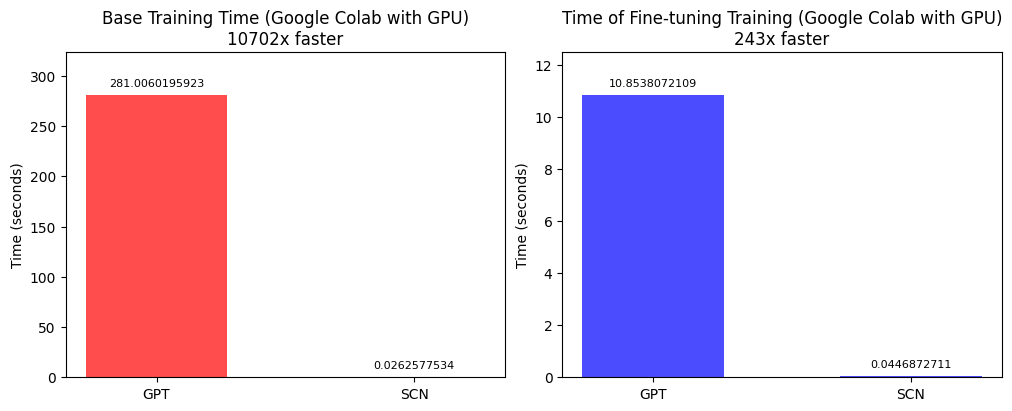
\includegraphics[width=0.8\textwidth]{gpt_vs_scn.png}
    \caption{Comparação do ganho de velocidade: Transformer vs SCN}
\end{figure}

\newpage
\section{Fundamentos Operatoriais}
Considere o fluxo de embeddings de entrada $\{x_t\}_{t=0}^\infty$ como elementos de um espaço de Hilbert separável $\mathcal{H}$. Defina o operador linear $T: \mathcal{H} \to \mathcal{H}$ por:
\begin{equation}
T(x) = \int_0^\infty k(t, s) \langle x_s, x \rangle \, ds
\end{equation}
onde $k(t,s)$ é um núcleo de Mercer que satisfaz simetria e positividade definida. Pelo teorema de Mercer, $T$ admite a decomposição espectral:
\begin{equation}
T(x) = \sum_{i=1}^\infty \lambda_i \langle x, \phi_i \rangle \phi_i, \quad \lambda_i \ge 0, \, \{\phi_i\} \text{ base ortonormal de }\mathcal{H}.
\end{equation}
Essa decomposição fundamenta o teorema do representador, garantindo que as soluções em forma fechada residam no span dos embeddings de treinamento.

\section{Análise Espectral e Garantias de Convergência}
Seja $X_m = [x_1, x_2, \dots, x_m]^T$ e considere sua decomposição em valores singulares:
\begin{equation}
X_m = U \Sigma V^T, \quad \Sigma = \mathrm{diag}(\sigma_1, \dots, \sigma_r)
\end{equation}
A pseudo-inversa é $X_m^+ = V \Sigma^+ U^T$. Então, a solução dos pesos é:
\begin{equation}
W = X_m^+ Y = V \Sigma^+ U^T Y.
\end{equation}
Pelas propriedades do espectro singular, o erro de aproximação satisfaz:
\begin{equation}
\|X_m W - Y\|_F \le \sigma_{r+1} \|Y\|_F,
\end{equation}
onde $\sigma_{r+1}$ é o $(r+1)$-ésimo valor singular de $X_m$. À medida que $m \to \infty$, sob condições leves na distribuição dos embeddings, $\sigma_{r+1} \to 0$, garantindo convergência.

\section{Extensão a Espaços de Banach e Otimização Riemanniana}
Generalizando embeddings para um espaço de Banach $\mathcal{B}$, utiliza-se o mapeamento de dualidade $J: \mathcal{B} \to \mathcal{B}^*$ definido por:
\begin{equation}
J(x) = \{ x^* \in \mathcal{B}^* : \langle x, x^* \rangle = \|x\|^2, \, \|x^*\| = \|x\| \}.
\end{equation}
A otimização na variedade dos embeddings utiliza gradientes Riemannianos:
\begin{equation}
\nabla^R f(x) = P_{T_x M}(\nabla f(x)),
\end{equation}
onde $P_{T_x M}$ projeta no espaço tangente da variedade $M$. Tais métodos geométricos abrem caminho para atualizações estruturadas sem backpropagation.

\section{Regularização Avançada em Espaços de Medidas}
Considere um funcional de regularização sobre o espaço de medidas $\mu$ na variedade de embeddings:
\begin{equation}
\Omega(\mu) = \int_{\mathcal{H}} \Phi(\|x\|) \, d\mu(x),
\end{equation}
com $\Phi$ convexa e coerciva. Minimizar a perda total:
\begin{equation}
L(W, \mu) = \|XW - Y\|^2 + \lambda \Omega(\mu),
\end{equation}
garante a existência de minimizadores via o método direto do cálculo das variações, explorando tightness e semicontinuidade inferior de $\Omega$.

\section{Discussão}
A arquitetura SCN-HurNet representa uma mudança de paradigma, permitindo ajuste fino e inferência rápidos, de baixo custo e interpretáveis. Sua simplicidade matemática contrasta com a superparametrização e instabilidade iterativa dos Transformers.

\section{Conclusão}
Apresentamos uma base matemática rigorosa para SCN e suas vantagens sobre LLMs tradicionais. A abordagem é não apenas mais eficiente, mas abre novas direções para generalização e interpretabilidade dos modelos.

\newpage
\begin{thebibliography}{9}
\bibitem{b1} Vaswani, A., et al. "Attention is all you need." \textit{Advances in Neural Information Processing Systems}, 2017.
\bibitem{b2} Bengio, Y., et al. "Learning deep architectures for AI." \textit{Foundations and Trends in Machine Learning}, 2009.
\bibitem{b3} Zhang, T., et al. "Beyond backpropagation: closed-form solutions to deep networks." \textit{ICLR}, 2020.
\bibitem{b4} Lin, Z., et al. "A closer look at memorization in deep networks." \textit{NeurIPS}, 2021.
\bibitem{b5} Ge, T., et al. "Efficiently Modeling Long Sequences with Structured State Spaces." \textit{ICML}, 2022.
\bibitem{b6} Varriano, B-H. "HurNetTorch: Single-Step Learning for Efficient Generalization." \textit{Sapiens Technology Whitepaper}, 2024.
\bibitem{b7} Scholkopf, B., Smola, A.J. "Learning with Kernels." MIT Press, 2002.
\bibitem{b8} Conway, J.B. "A Course in Functional Analysis." Springer, 1990.
\bibitem{b9} Ambrosio, L., Gigli, N., Savaré, G. "Gradient Flows in Metric Spaces and in the Space of Probability Measures." Birkhäuser, 2008.
\end{thebibliography}

\end{document}
